\documentclass[a4paper,english, 10pt, twoside]{article}
\usepackage[utf8]{inputenc}
\usepackage[T1]{fontenc}
\usepackage[english]{babel}
\usepackage{epsfig}
\usepackage{graphicx}
\usepackage{amsfonts, amssymb, amsmath}
\usepackage{listings}
\usepackage{float}
\usepackage[top=2cm, bottom=2cm, left=2cm, right=2cm]{geometry}
%\newcommand{\d}{\partial}
%opening
\title{Project 4, FYS4150}
\author{Fredrik E Pettersen\\ fredriep@student.matnat.uio.no}


\begin{document}

\maketitle


\section*{About the problem}

\section*{The algorithm}

\section*{Analytic solution}
As a comparison we can find the analytic solution to this problem as follows. 
 \begin{align}\label{eq}
  &\frac{\partial u}{\partial t} = D\frac{\partial^2 u}{\partial x^2}, \,\,\,\,\, u(x,0) = u(d,t) = 0\\
  &x\in[0,d],\,\,\,\,\,\, D = d = u(0,t) = 1
 \end{align}
We see right away that the boundary $x=0$ could give us some problems, so we start off with a small trick
$$
u(x,t) = v(x,t) = u(x,t) - u_s(x)
$$
where the $u_s = 1-x$ term is the steady-state solution to equation \ref{eq}. This trick leaves us with new boundary conditions 
un $u(x,t)$ 
$$
v(0,t) = u(0,t) - u_s(0,t) = 1, \;\; u_s(0,t) = 1 \implies u(0,t) = 0
$$
which makes the whole procedure much simpler. We now assume that $u(x,t)$ can be separated into factors 
\begin{align*}
&u(x,t) = F(x)G(t) \implies \frac{\partial u}{\partial t} = \frac{\partial^2 u}{\partial x^2} \to F(x)\frac{\partial G}{\partial t}
= G(t)\frac{\partial^2 F}{\partial x^2}\\
&\frac{1}{G(t)}\frac{\partial G}{\partial t} =-k^2 =  \frac{1}{F(x)}\frac{\partial^2 F}{\partial x^2}
\end{align*}
We start with the simplest of the equations which is the time dependence
\begin{align*}
 \frac{1}{G(t)}\frac{\partial G}{\partial t} =-k^2\\
 G(t) =C e^{-k^2t}
\end{align*}
and leave it like this for now. The x-dependent equation is somewhat more complicated
\begin{align*}
 \frac{1}{F(x)}\frac{\partial^2 F}{\partial x^2} = -k^2 \\
 F(x) = A\sin(kx) + B\cos(kx)
\end{align*}
\begin{align*}
 F(0) = A\sin(0) + B\cos(0) = 0 \implies B= 0\\
 F(d) = A\sin(kd) = 0 \implies k = \frac{m\pi}{d} = \pi m, \;\; A = A_m
\end{align*}
we now combine all the equations to determine $v(x,t)$
\begin{align*}
 v(x,t) = 1-x + \sum\limits_{m=1}^{\infty}B_me^{-(m\pi)^2t}\sin(m\pi x) \\
 v(x,0) = 1-x +\sum\limits_{m=1}^{\infty}B_m\sin(m\pi x)\\
 \implies \int\limits_0^1\sin(m\pi x)\sin(n\pi x)dx = \delta_{mn} = \int\limits_0^1(x-1)\sin(m\pi x)dx = -\frac{2}{m\pi} = B_m
\end{align*}
This gives us the full analytical solution 
\begin{equation}\label{solution}
 v(x,t) = 1-x-\frac{2}{\pi}\sum\limits_{m = 1}^{\infty}\frac{1}{m}e^{-(m\pi)^2t}\sin(m\pi x) 
\end{equation}
which satisfies all initial and boundary conditions.
\section*{Results}


\section*{Stability and precision}

% \begin{figure}[H]
%  \centering
%  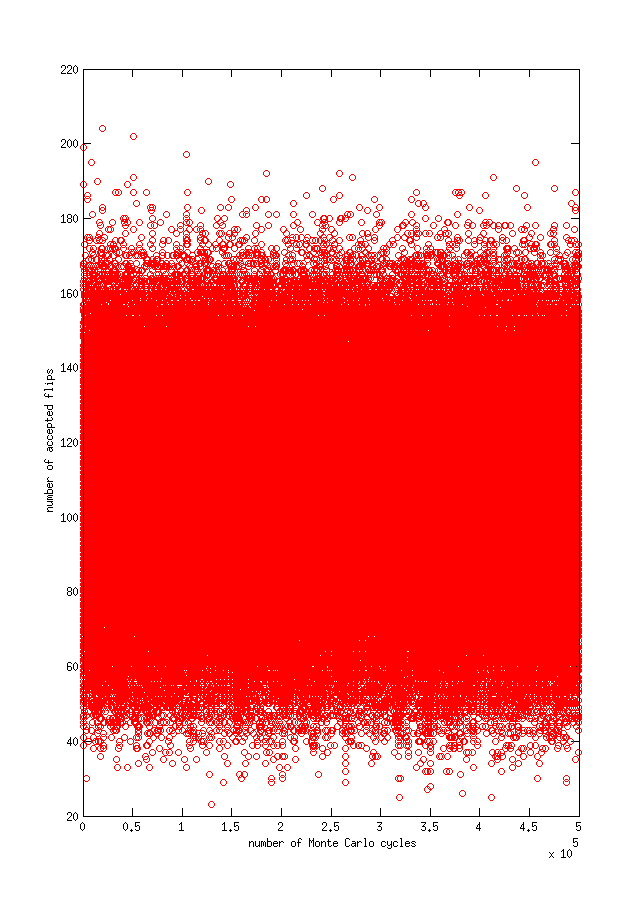
\includegraphics[scale = 0.45]{accepted_flips_temp2dot4.png}
%  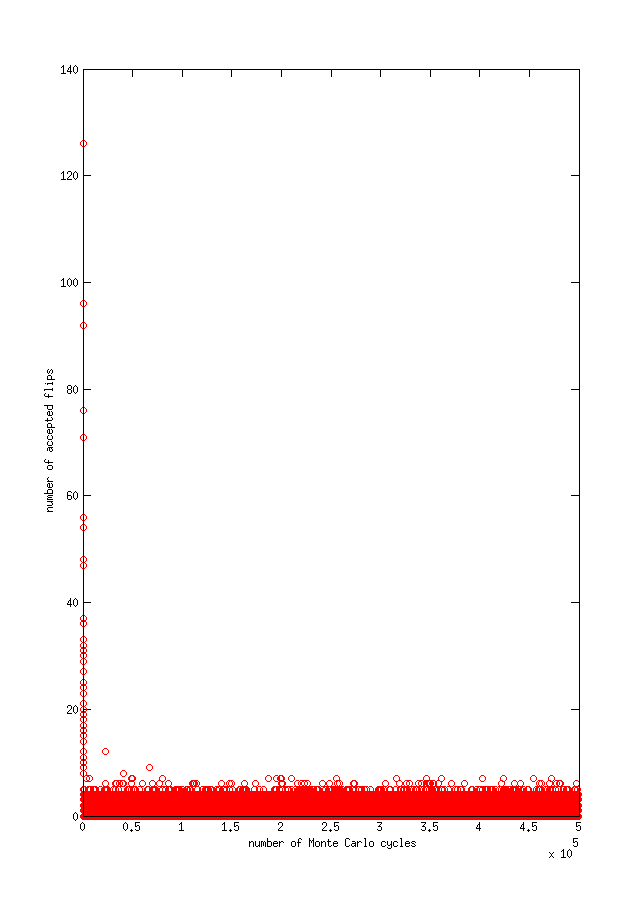
\includegraphics[scale = 0.45]{accepted_flips_temp1.png}
%  \caption{Number of accepted spin flips. T = 2.4 to the left, and T = 1 on the right.}
%  \label{both_accepted_flpis}
% \end{figure}
\section*{Final comments}

\end{document}
